\documentclass{math}

\usepackage{enumerate}
\usepackage{graphicx}

\title{Intro to Computer Science Theory: Homework 5}
\author{Alvin Lin and Joshua Cotton}
\date{August 2017 - December 2017}

\begin{document}

\maketitle

\subsection*{Problem 1}
Use the so-called \textit{subset construction} given in Theorem 1.39 to
draw state transition diagrams for (D)FAs for each of the NFAs below. Name the
states of the FA so that for each it is clear which subset of NFA states it
represents. You need only show the states that are reachable from the initial
state.
\begin{enumerate}[(a)]
  \item
  \begin{center}
    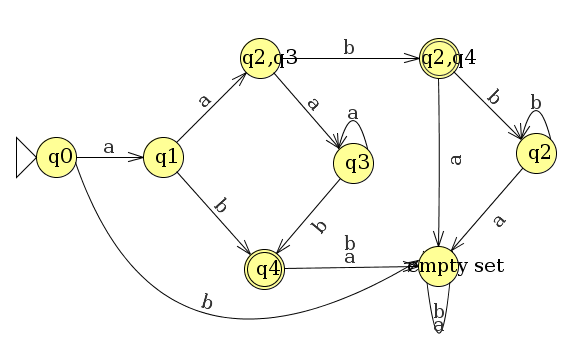
\includegraphics[width=15cm]{assets/hw_5_1.png}
  \end{center}
  \item
  \begin{center}
    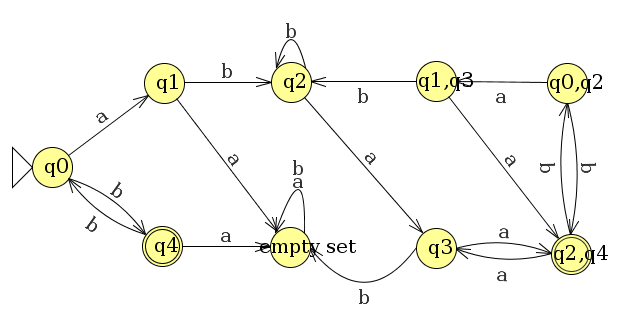
\includegraphics[width=15cm]{assets/hw_5_2.png}
  \end{center}
\end{enumerate}

\subsubsection*{Problem 2}
Choose one of the following NFAs from above and:
\begin{enumerate}[(a)]
  \item give a formal definition of the NFA. You may rename the states if that
  makes your definition clearer or more elegant, but if so you must either
  redraw the machine or indicate how the old names map to the new names.
  \begin{align*}
    M &= \{Q,\Sigma,\delta,q_0,F\} \\
    Q &= \{q_0,q_1,q_2,q_3,q_4\} \\
    \Sigma &= \{a,b\} \\
    \delta(q,x):Q\times\Sigma\to2^{Q} &= \begin{tabular}{|c|cc|}
      \hline
          & a                 & b               \\ \hline
      \( q_0 \) & \( \{q_1\}     \) & \( \emptyset \) \\ \hline
      \( q_1 \) & \( \{q_2,q_3\} \) & \( \{q_4\}   \) \\ \hline
      \( q_2 \) & \( \emptyset   \) & \( \{q_2\}   \) \\ \hline
      \( q_3 \) & \( \{q_3\}     \) & \( \{q_4\}   \) \\ \hline
      \( q_4 \) & \( \emptyset   \) & \( \emptyset \) \\ \hline
    \end{tabular} \\
    q_0 &= q_0 \\
    F &= \{q_4\}
  \end{align*}
  \item give a formal definition for the FA equivalent to the NFA you did not
  choose. You may rename the states if that makes your definition clearer or
  more elegant, but if so you must either redraw the machine or indicate how
  the old names map to the new names. Your definition must stand in its own way
  and may not refer to the NFA on which it is based.
  \begin{align*}
    M &= \{Q,\Sigma,\delta,q_0,F\} \\
    Q &= \{q_0,q_1,q_2,q_3,q_4,q_1q_3,q_0q_2,q_2q_4,\emptyset\} \\
    \Sigma &= \{a,b\} \\
    \delta(q,x):Q\times\Sigma\to Q &= \begin{tabular}{|c|cc|}
      \hline
                   & a               & b               \\ \hline
      \( q_0    \) & \( q_1       \) & \( q_4       \) \\ \hline
      \( q_1    \) & \( \emptyset \) & \( q_2       \) \\ \hline
      \( q_2    \) & \( q_3       \) & \( q_2       \) \\ \hline
      \( q_3    \) & \( q_2q_4    \) & \( \emptyset \) \\ \hline
      \( q_4    \) & \( \emptyset \) & \( q_0       \) \\ \hline
      \( q_1q_3 \) & \( q_2q_4    \) & \( q_2       \) \\ \hline
      \( q_0q_2 \) & \( q_1q_3    \) & \( q_2q_4    \) \\ \hline
      \( q_2q_4 \) & \( q_3       \) & \( q_0q_2    \) \\ \hline
    \end{tabular} \\
    q_0 &= q_0 \\
    F &= \{q_4,q_2q_4\}
  \end{align*}
\end{enumerate}

\begin{center}
  If you have any questions, comments, or concerns, please contact me at
  alvin@omgimanerd.tech
\end{center}

\end{document}
